\documentclass{article}
\usepackage[UTF8]{ctex}
\usepackage{geometry}
\usepackage{multirow}
\usepackage{natbib}
\geometry{left=3.18cm,right=3.18cm,top=2.54cm,bottom=2.54cm}
\usepackage{graphicx}
\pagestyle{plain}	
\usepackage{setspace}
\usepackage{enumerate}
\usepackage{caption2}
\usepackage{datetime} %日期
\renewcommand{\today}{\number\year 年 \number\month 月 \number\day 日}
\renewcommand{\captionlabelfont}{\small}
\renewcommand{\captionfont}{\small}
\begin{document}

\begin{figure}
    \centering
    
\includegraphics[width=8cm]{upc.png}

    \label{figupc}
\end{figure}

	\begin{center}
		\quad \\
		\quad \\
		\heiti \fontsize{45}{17} \quad \quad \quad 
		\vskip 1.5cm
		\heiti \zihao{2} 《计算科学导论》个人职业规划
	\end{center}
	\vskip 2.0cm
		
	\begin{quotation}
% 	\begin{center}
		\doublespacing
		
        \zihao{4}\par\setlength\parindent{7em}
		\quad 

		学生姓名:\underline{\qquad  李保辉 \qquad \qquad}

		学\hspace{0.61cm} 号:\underline{\qquad 1907010120\qquad}
		
		专业班级:\underline{\qquad 计科1901 \qquad  }
		
        学\hspace{0.61cm} 院:\underline{计算机科学与技术学院}
% 	\end{center}
		\vskip 1.5cm
		\centering
		\begin{table}[h]
            \centering 
            \zihao{4}
            \begin{tabular}{|c|c|c|c|c|c|c|c|c|}
            % 这里的rl 与表格对应可以看到,姓名是r,右对齐的;学号是l,左对齐的;若想居中,使用c关键字。
                \hline
                \multicolumn{5}{|c|}{分项评价} &\multicolumn{2}{c|}{整体评价}  & 总    分 & 评 阅 教 师\\
                \hline
                自我 & 环境 & 职业 & 实施 & 评估与 & 完整性 & 可行性 &\multirow{2}*{} &\multirow{2}*{}\\
                分析& 分析& 定位 & 方案 & 调整 & 20\% & 20\% & ~&~ \\\            
                10\% & 10\% & 15\% & 15\% & 10\% & &  &~ &~\\
                \cline{1-7} 
                & & & & & & & ~&~ \\
                & & & & & & & ~&~ \\
                \hline      
            \end{tabular}
        \end{table}
		\vskip 2cm
		\today
	\end{quotation}

\thispagestyle{empty}
\newpage
\setcounter{page}{1}
% 在这之前是封面,在这之后是正文
\section{自我分析}
	这是我来到大学的第一个学期,我深深的感受到了大学的活力。在这个学期,我初步了解了一门语言,而且还学会了使用一些其他的软件。不过,我感觉到我的学习方式还是不够完善,并且自身还有多方面的缺点。比如,(1)无法合理安排自己的时间,不能很好的利用自己的空闲时间。(2)在上课时无法很好的集中注意力,并且无法合理安排自己的作息时间,不能做到合理作息。(3)我的学习方式还处于高中阶段,没有制定出适合大学的学习方式。(4)我的各方面的能力都有待提高,特别是人际交往能力。

    除此之外,我的性格也比较内向。我感觉我一直活在自己的世界之中,并且我经常性的尽量回避与他人交流。
    
    对于我的兴趣,我也没有什么明确的兴趣。不过我个人还是挺喜欢与未来有关的事情。比如,人工智能,鸿蒙操作系统,物联网。但是,我不好的是,我虽然对他们感兴趣但是我并没有去深入的去了解这些东西,只是在听老师说其实我感觉特别的向往。

    而且,我对于我自己将来想要做什么并没有很明确的目标。我也希望我可以在大学的四年中全面的改善自己,努力提高个人实力,找到自己真正喜欢做的事业,明确自己的目标,找到自己真正感兴趣的事情或是方面。\par
\par\subsection{自然条件}
    性别男,刚到18周岁,身体方面没有什么特别突出的,身体健康,老家在山西省临汾市隰县,目前正在山东省青岛市黄岛区长江路西路66号中国石油大学(华东)上大学。\par
\subsection{性格分析}
    我个人认为我比较的内向,我不喜欢人多的地方,我经常感觉到自己一个人就好。同时我也是一个不善于表达自己人,我害怕在大众面前发言,主要是我从小就缺少自信,并且由于我高中的学习模式我没有去注意自己的性格。但是,当我到达大学后我深深的认识到了我性格方面从在的缺陷。我虽然对于高水平没有太大的追求,但是,我对于自己努力就可以做到的事情我会想办法去实现它。\par
\subsection{教育与学习经历}
    对于我的教育和学习经历,我个人感觉就是十分的平常。但是,大多数的时候都是老师布置了任务我才去做。因此,我没有主动学习的意识,我也不会去合理的安排时间。因此我一直处于被动学习的过程中,等到了大学我意识到了这种被动学习的坏处。但是,当我想要去改变的时候我发现我没有对应的方法去改变。但是,我在接下来的学习过程中我会尽量的慢慢的改变自己被动的学习。\par
\subsection{工作与社会阅历}
    我的工作与社会阅历可以说几乎为零,这主要与我的经历有关。我大多数时间都是在学校里度过的,对于社会上的事情接触的不是很多。虽然我在暑假的时候打过工。但是,并没有和太多的人接触过,因此我也没有得到较多的经验。所以,我的阅历可以说是没有。这也间接导致我的人际交往能力严重下降。\par
\subsection{知识、技能与经验}
    就目前而言,我的知识面还处于学习的阶段,基本只了解学习过的知识。然而对于那些课外的知识我可以说是一概不了解。对于技能方面,我只是了解一些基本操作谈不上什么技能。除此之外,我对于课外的东西没有什么经验。\par
\subsection{兴趣爱好与特长}
    由于我刚兴趣的方面的太多导致我也无法明确自己的兴趣到底是什么样的。关于我的特长,我认为我的特长就是可以快速适应新的环境。我可以很快的适应不同的人和环境,并且可以根据环境的不同来调整自己。只是我无法快速的进行调整,只能在环境中慢慢的进行改进。\par
\section{环境分析}
环境分析包括:\par
\subsection{社会环境分析}
     中国现在正处于近两百年以来最好的历史时期。虽然社会上还有许多的体制弊端,还有许多没有解决的矛盾,但是政治上比较稳定,法制化进程已经开始,市场经济已经初步形成并步入正轨。二十一世纪的中华大地充满各种人才成长发展的机遇。

     但是我们也要看到,人才的竞争日趋激烈,大学生就业难、失业率居高不下等等,都使我们的就业环境看起来不容乐观。因此,我们就更应该根据目前的社会环境来做好自己的职业规划。

     总体来说,我们现在面临一个非常好的宏观环境,社会安定,政治稳定,经济发展迅速,并与全球一体化接轨,法制建设不断完善,文化繁荣自由,尖端技术、高新技术突飞猛进。因此,在这个大前提之下,我们需要特别注意的是职业环境的变化。\par
\subsection{家庭环境分析}
    总的来说我的家庭还是挺好的,因为,无论发生了什么父母他们都会尊重我的意见。并且,即使他们之间发生了争执他们也会因为我而和好。    

    虽然我们家庭经济并不是很富裕,并且我上大学时也贷了款。但是,我们也是有自己家的房子、车。并且,我们对日常的温饱不用担心。只是因为家中除了我这个大学生以外还有一个上初中的弟弟。所以,我的父母还是省吃俭用的,而我也受到了他们的影响我基本上除了一日三餐外几乎不吃零食。而且,我也不会在网上买一些无关紧要的东西。并且,我们一家人几乎都是不到过年并不买新衣服的那种。

    而且,由于我是我爸和我妈两边第一个考上大学的孩子。因此,我父母对我的期望很高,并且他们也十分的理解我,尽量不给我施加太多的压力。我对于有这样的父母感到幸运和感激。

    对于家中的传统我了解的并不是很多,因为,我们并没有什么家族的概念所以我们家中并没有什么与别人家不一样的传统。\par
\subsection{职业环境分析}
	\subsubsection{ 行业现状及发展趋势}

随着科学技术的持续深入发展和我国经济水平不断提高,计算机的普及程度也在迅速扩展,计算机应用技术已经被广泛应用到各行各业中,并为这些行业的发展带了史无前例的推动作用。随着科学技术的持续深入发展和我国经济水平不断提高,计算机的普及程度也在迅速扩展,计算机应用技术已经被广泛应用到各行各业中,并为这些行业的发展带了史无前例的推动作用。
	\subsubsection{ NET 高级软件工程师 }

工作内容:

          1、 参与系统的需求分析、架构设计,负责重要模块开发编码 

          2、 对中级程序员能起到指导作用,通过各种途径高效解决技术问题 

          3、 参与数据库设计,熟练使用Power Designer等建模工具

工作要求:

          1、计算机及相关专业本科以上 

          2、2年以上IT行业工作经验,至少1年以上的ASP.NET开发经验 

          3、精通C\#,XML,JavaScript,HTML,有WinForm开发经验 

          4、熟悉面向对象分析和设计(OOAD),统一建模语言(UML) 

          5、精通SQL Server、VSS、PD、ROSE等开发、设计和管理工具

          6、具备一定的口头和书面表达能力,能够撰写软件分析和设计方案 

          7、具备一定的沟通协调能力以及团队合作精神,有责任心、有创业激情 

          8、有ERP或其他大型管理软件开发经验者优先
	\subsubsection{ 前景:}

\begin{enumerate}[(1)]
	\item 首先,人才需求量大。我们来看一个数据,据有关权威部门统计,将来几年内我国软件行业的从业机会十分庞大,每年对软件人才的需求将达到35万-40万人,而每年高校培养出来的计算机相关专业的毕业生只有6万人左右。
	\item 其次,较高的就业薪水。据几位业内人士透露,以一线操作为主的从业人员每月工资应在3000元至6000元左右,在北京地区,职业教育软件相关专业的学生每月平均收入可达到五千元左右,而具有一定工作经验的编码人员的月薪就可高至八九千元。他们说,与其成为一个“平庸的管理者”,不如成为一名“出色的操作者”,因此,软件工程师自然是前途无量。
	\item 再次,用人单位需求旺盛,用人单位对.net软件工程师的需求可以用“如饥似渴”来形容,用人单位中很多是银行的IT部门和跨国IT企业,对于具有实际操作能力的软件人才是用人单位为需要的,而且越是上规模的公司,工作的拆分层次越清晰,对于软件人才的需要越大。
	\item 最后,软件工厂有大量需求量。据有关部门了解,由于人才严重不足,很多企业不得不从软件人才的培训做起,随着来自印度的IT培训被耳熟能详时,更有重金招募的信息地激起人们对该职业的向往。
\end{enumerate}
\par 
\par 

\subsection{地域与人际环境分析}
 
\subsubsection{气候水土}
    青岛地处北温带季风区域,属温带季风气候,略有海洋性气候特征.市区由于海洋环境的直接调节,受来自洋面上的东南季风及海流、水团的影响,故又具有明显的海洋性气候特点.空气湿润,温度适中,四季分明.春季气温回升缓慢,较内陆迟1个月;夏季湿热多雨,但无酷暑7月平均温度23度,极端高温37.4度;秋季天高气爽,降水少;冬季风大温低,持续时间较长,但并无严寒,1月平均温度-3度,极端低温-16度.

    据1898年以来百余年气象资料查考,市区年平均气温12.7摄氏度,极端高气温38.9摄氏度(2002年7月15日),极端低气温-16.9摄氏度(1931年1月10日).全年8月份最热,平均气温25.3摄氏度;1月份最冷,平均气温-0.5摄氏度.日最高气温高于30摄氏度的日数,年平均为11.4天;日最低气温低于-5摄氏度的日数,年平均为22天.降水量年平均为662.1毫米,春、夏、秋、冬四季雨量分别占全年降水量的17\%、57\%、21\%、5\%.年降水量最多为1272.7毫米(1911年),最少仅308.2毫米(1981年),降水的年变率为62\%.年平均降雪日数只有10天.年平均气压为1008.6毫巴.年平均风速为5.2米/秒,以南东风为主导风向.年平均相对湿度为73\%,7月份最高,为89\%;12月份最低,为68\%.
\par 
\begin{figure}[h!]
\centering
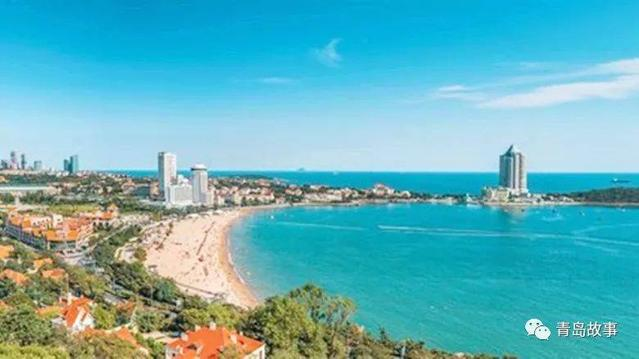
\includegraphics[scale=0.25]{jingsetupian}
\caption{}
\label{fig:jingsetupian}
\end{figure}

\subsubsection{文化特点}

\begin{enumerate}[(1)]
	\item 青岛是一个地地道道的移民城市,90\%以上的居民来自于四面八方;青岛是一个浸染着外来文化的城市,就连方言里都嵌刻着外来的印记,“你这个负儿”其实就是英文里的“fool”,“白痴”、“笨蛋”的意思,“你看你杠杠的”就是“ganglike”的谐音,意指“像个流氓”,“搓牌”就是strawberry的谐音草莓,还有“扎古扎古”就是日语修理的谐音,“赤鳞”“涨颠”是德语狂妄、傲慢的意思;青岛是一个万国建筑博览会,德式的、日式的、葡式的、俄式的、西班牙式的,还有伊斯兰式的,甚至还有不同风格不同教派的教堂;青岛是一个文化名人聚集区,康有为、梁启超、老舍、王统照、闻一多、萧军、萧红等等,都曾经在青岛留下了他们的足迹......
	\item 所以,有人俗称青岛文化是“两活水”的文化。就是这“两活水”的文化,塑造了青岛人那特有的性格和气质——自大而又自信,聪慧而又豪爽,算计而又大方,保守而又开放,故土难舍而又海纳百川。
	\item 青岛虽被称为文化沙漠,却又有音乐之城、足球之城、时装之城、建筑之城、奥帆之城的美誉,在全国诸多文明城市评选中,青岛位居榜首......
	\item 青岛的文化很另类,青岛的文化很现代。青岛的文化恰如那片广阔无垠的湛蓝,容纳着来自四面八方的滔滔激流和潺潺细水;恰如她音乐之城的美誉,演绎着一曲富有现代韵律的社会发展的交响乐章。
\end{enumerate}

\begin{figure}[h!]
\centering
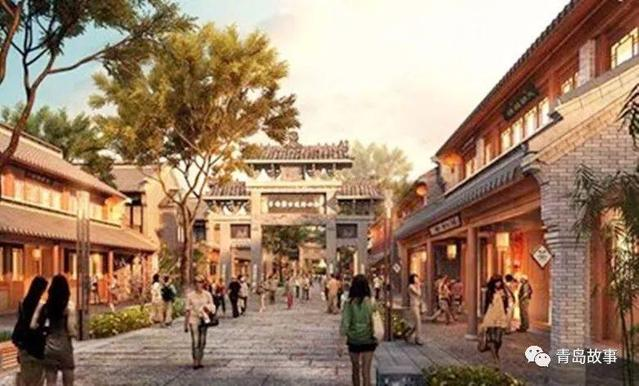
\includegraphics[scale=0.25]{wenhua}
\caption{}
\label{fig:wenhua}
\end{figure}

\subsubsection{发展前景}

\begin{enumerate}[(1)]
	\item 青岛所处的山东板块位于我国南北两最大直辖市为核心的大城市群中间地带,一条胶济铁路贯穿起济青为两端的经济文化隆起带,把青岛与中国这两大城市群相连。以海空运输通联世界,这造就了青岛区域核心和枢纽角色。
	\item 未来这方面的地位还会继续加强,南北沿海铁路填补了青岛历史上的一个大的短板,带来了青岛西站这个可以始发终到的大站。航空会在胶东机场使用后快速强化枢纽作用,海运也不会落后,排不到第一也必是前列,公路自不必说,早已成枢纽型。
    \item 青岛不光拥有湾岬相间、散罗众多沙滩和小山的唯美前海主城区,还独自享有一个中小型的海湾——胶州湾,和一条十分曲折的海岸线。新的城市发展规划把这一切都充分纳入,发展空间完全打开,有条件吸纳大量人口和资源。一座海湾型城市前景是可以预见的。
	\item 产业方面,青岛历来有积极培植制造业的传统,也成功一些,形成一批有一定特色的,国内有一定影响力的品牌和产业。重工业一直是相对短板,也在逐步补齐。未来在科技创新和奢侈品开发方面应该加强,生活水平的提高,让中国人有了更高的物质需求和对外辐射影响力的能力,奢侈品也是品牌化的产物,需要精尖制造。这方面南方城市无疑有更大的优势,过去的山寨,现在的A货都为他们打下了基础。
	\item 文旅业一直是青岛较为著名的,将来会继续走唯美与文艺路线,随着老城区的整治和开发,将为来青岛发展和旅游休闲的人们端上一桌十分优美的大餐。蜿蜒曲折的海岸线慢行系统的建设,会使青岛成为一个特别亲海的城市,海景房不再稀缺,大不了想看海,走两步。
\end{enumerate}

\section{职业目标}

\subsection{成果目标}
\begin{enumerate}[(1)]
\item在毕业后基本达成该职业的大多数学习要求
\end{enumerate}
\par
\subsection{经济目标}
\begin{enumerate}[(1)]
\item在进入工作3到5年可以有一个可观并且稳定的收入
\end{enumerate}
\par
\subsection{能力目标}
\begin{enumerate}[(1)]
\item在毕业后各方面能力可以全面提升到预期目标,在进入工作后1到3年内使职业知识得到全面补充。
\end{enumerate}
\par
\subsection{职务目标}
\begin{enumerate}[(1)]
\item可以有自己的办公空间。
\end{enumerate}
\par

\section{实施方案}
\begin{enumerate}[1]
	\item 尽可能利用身边师资资源,使自身的优势可以得到全面利用
	\item 合理控制时间,不断调整自己的学习方式,尽可能的通过图书馆、老师、同学、网络来了解更多知识
	\item 多读一些有关如何待人处事的书籍,提高自己的沟通能力,尽可能结交更多的人才。
	\item 在空闲时间出去看会书或是到周边城市去逛逛,或是和朋友出去一起玩
\end{enumerate}
\par 

\section{评估与调整}

\subsection{评估时间}
在没学期末时进行一次评估\par
\subsection{评估内容}
看自己是否在逐渐接近目标,看对比以前是否有较大的提升。\par
\subsection{调整原则}
结合自身的改变情况具体进行调整\par




\end{document}
